\documentclass[12pt]{article}
\usepackage{graphicx}
\usepackage{amsmath}
\usepackage[utf8x]{inputenc}
\usepackage[T1]{fontenc}
\usepackage{url}
\usepackage{caption}
\usepackage{palatino}
\usepackage[paper=a4paper,margin=2cm,bmargin=3cm]{geometry}
%\usepackage[turkish]{babel}
\author{M. Atakan Gürkan}
\title{Çizelgenin Kullanımı}
\date{}
\begin{document}
\maketitle
\section{Genel açıklamalar}
Bu çizelge 2012 yılı için Ankara'da çeşitli gök cisimlerinin doğma,
meridyenden geçme (bkz. Şekil 1) ve batma zamanlarını,
alacakaranlığın sonuyla başlangıcını ve Ay'ın evrelerini gösteriyor.
\begin{figure}
  \label{fig:meridyen}
  \begin{center}
    \begin{minipage}[t]{0.6\textwidth}
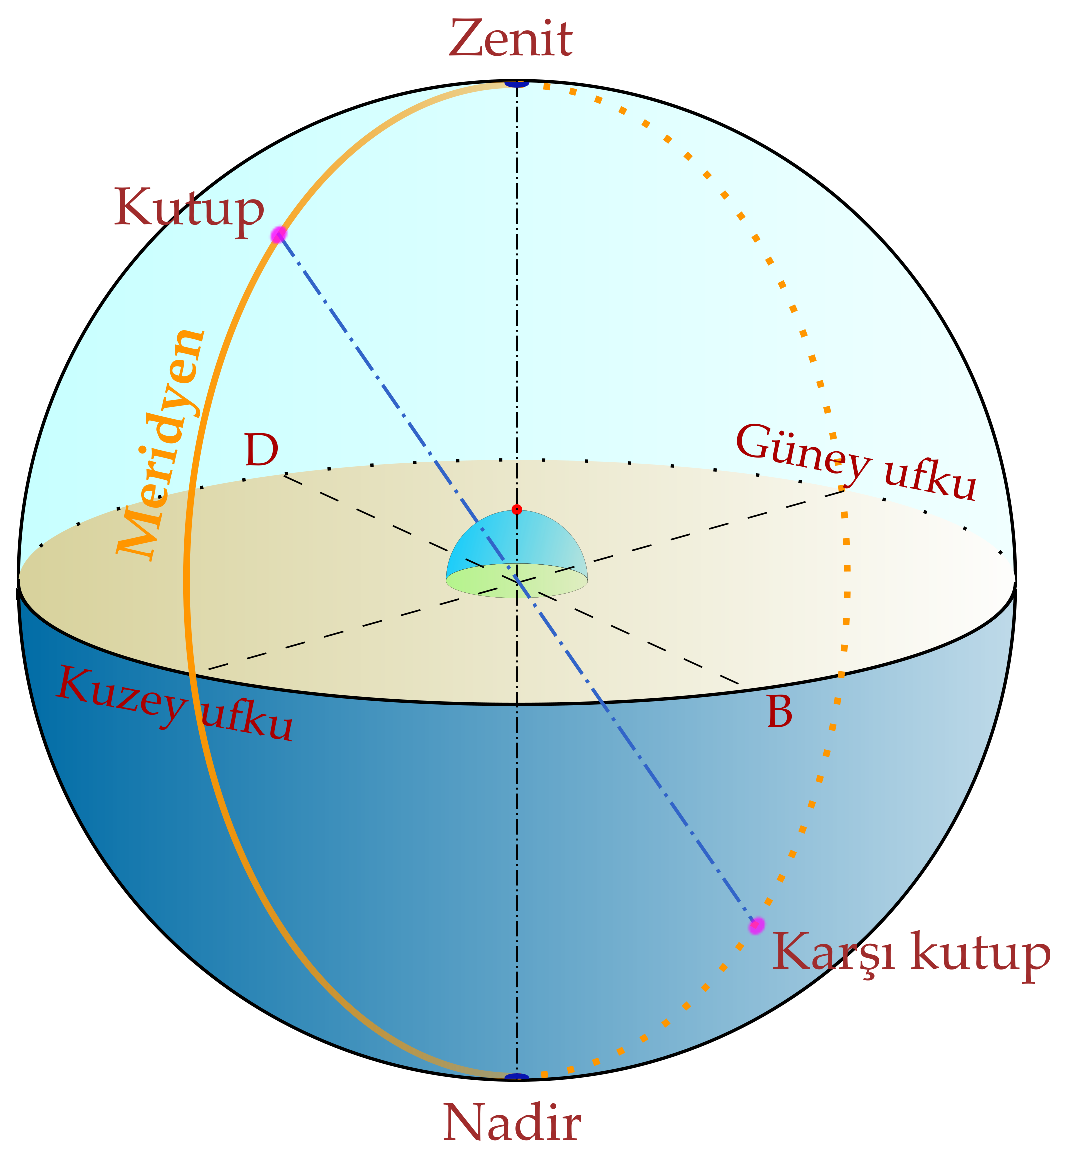
\includegraphics[width=\textwidth]{Meridyen}
    \end{minipage}\hfill
    \begin{minipage}[b]{0.38\textwidth}
\caption*{\textbf{Şekil 1.} Gökyüzünde meridyenin ve kerteriz noktalarının gösterimi. Meridyen,
gökyüzünde tepe noktası zenitten ve gökyüzünün çev\-re\-sin\-de dönüyor gibi
göründüğü kutup noktasından geçen, ufku dik kesen bir çemberdir. Gök
cisimleri ufuktan en yüksek ve en alçak noktalarına, genel olarak,
meridyenden geçerken ulaşır.}
    \end{minipage}
  \end{center}
\end{figure}

Dikey eksen günleri, yatay eksen gece boyunca zamanı göstermektedir.
Gece içinde yarımşar saatlik aralıklar ve yıl içinde Pazar akşamlarını
Pazartesi sabahlarına bağlayan geceler noktalı çizgilerle
belirtilmiştir; düşey olarak iki nokta arası bir güne, yatay olarak iki
nokta arası beş dakikaya karşılık gelir.

Belli bir gecede neler olacağı, çizelge üzerinde sol tarafta o
geceye karşılık gelen nokta bulunup, sağa doğru ilerleyerek
görülebilir.  Bir örnek olarak 13 Mart gecesinin olaylarına
bakalım. İlk olarak, sol tarafta 11 Mart'a karşılık gelen
noktanın altında yaklaşık olarak 13 Mart'a karşılık gelen
noktayı bulalım. Buradan sağa doğru ilerlediğimizde ilk
gördüğümüz 18:00'e bir kaç dakika kala Avcı Bulutsusu'nun
ve hemen ardından 18:15 civarında Betelgeuse'ün meridyenden
geçeceği. Daha sonra 18:40 civarında önce Uranüs, daha sonra
19:00 civarında da Merkür batıyor. Bu bilgilerden aynı zamanda
Güneş battığı zaman bu cisimlerin ufkun üzerinde olduğunu
da anlıyoruz. Sağa doğru ilerledikçe, belli saatlerde pekçok
gökcisminin doğduğunu, battığını ve meridyenden geçtiğini
görüyoruz. Geceyarısını 7-8 dakika geçe gördüğümüz Ay
sembolü, Ay'ın doğuş zamanını gösteriyor ve bir sonraki gece
Ay'ın daha küçük olacağını belirtiyor. Son olarak 19:25
ve 4:30 civarında gördüğümüz kesikli çizgiler sırasıyla
alacakaranlığın bitmesi ve başlamasını belirtiyor. Bu noktalar
Güneş'in ufkun 18$^\circ$ altında kaldığı anlara karşılık
geliyor.

Çizelgedeki doğma ve batma zamanları, ufuk çizgisinin önünde bir engel
olmadığı varsa\-yılarak yapılmıştır. Eğer böyle bir engel varsa, her bir
açı derecesi yükseklik için doğma zamanı 4 dakika geç, batma zamanı da
aynı miktarda erken olacaktır. Benzer biçimde, yüksek bir noktadan gözlem
yapıldığı için ufuk çizgisi olması gerekenin altında ise, doğma ve batma
zamanlarının düzeltilmesi gerekir.

\section{Yaz saati uygulaması}
Çizelgede sürekliliğin korunması için yaz saati uygulaması
dikkate alınmamıştır. Yaz saati uygulamasının geçerli olduğu
zamanlarda çizelgede okunan saatlere bir saat eklemek gerekmektedir.
Türkiye'de yaz saati Mart ayının son Pazar gününden, Ekim ayının
son Pazar gününe kadar uygulanır.

\section{Çizelgenin Ankara'dan başka yerlerde kullanımı}
Bu çizelge basit bir takım düzeltmelerle çok kuzey ya da çok güneye
gitmemek şartıyla Ankara (39.88$^\circ$ Kuzey,  32.81$^\circ$ Doğu)
dışındaki yerlerde de kullanılabilir.  Ankara'nın do\-ğu\-sun\-daki
noktalarda çizelgede verilen olaylar daha erken, batısındaki
noktalarda daha geç olacaktır. Aradaki zaman farkı herbir boylam
derecesi için 4 dakikadır.

Örneğin Ankara ile hemen hemen aynı enlemde ama daha doğuda olan
Erzurum (39.9$^\circ$ Kuzey,  41.27$^\circ$ Doğu) için çizelgede
belirtilen zamanlardan 34 dakika çıkartmak, benzer bi\-çimde
Çanakkale (40.09$^\circ$ Kuzey,  26.24$^\circ$ Doğu) için 26 dakika
eklemek gerekmektedir.

Kuzey ya da güney yönünde gidildikçe gökcisimlerinin
meridyenden geçme zamanı değişmese de, doğma ve batma
zamanları değişebilir. Bu değişimin büyüklüğü o cismin
kutup noktasından uzaklığına\footnote{Bu uzaklık cismin
dikaçıklığının 90 dereceden çıkarılmasıyla bulunabilir.}
bağlıdır. Türkiye'de ve genel olarak Kuzey yarımkürede,
güneye inildikçe cisimler gök\-yü\-zün\-de daha uzun kalırlar;
yani erken doğup, geç batarlar. Kuzeye gidildikçe de bunun tersi
olur. Örneğin 13 Mart gecesi Satürn Ankara'da 20:40'da, Anamur'da
(36.01$^\circ$ Kuzey, 32.48$^\circ$ Doğu) 20:35'te doğacaktır.

\section{Çizelgenin 2012 yılı dışında kullanımı}
Güneş Sistemi dışındaki yıldızların ve gökcisimlerinin yıldan yıla
konumları çok fazla de\-ğiş\-me\-di\-ği için, bu çizelge bu nesneler için 2012
yılı dışında da kullanılabilir. Bir yılın tam $365$ değil $365,25$ yıl
olmasından dolayı ortaya çıkacak oynamalar çok küçük olacaktır.
Gezegenler ve Ay için verilen zamanlar yalnız  2012 yılı için
geçerlidir.

\section*{Kaynaklar}
\begin{itemize}
\item Bu çizelge\\
\url{https://github.com/atakan/PySkyAlmanac}\\
adresindeki \texttt{PySkyAlmanac} programı kullanılarak hazırlanmıştır.
Bu program\\
\texttt{Xephem}, \texttt{Python}, \texttt{PyX}
\texttt{PyEphem} ve \texttt{SciPy} kütüphanelerini kullanmaktadır.
\item Meridyen resmi Wikimedia Commons'taki\\
\url{http://commons.wikimedia.org/wiki/File:Meridiano.svg}\\
dosyasından uyarlanmıştır.
\end{itemize}

\end{document}
